% !TeX spellcheck = de_DE
\chapter{\IfLanguageName{dutch}{Stand van zaken}{State of the art}}
\label{ch:stand-van-zaken}

% Tip: Begin elk hoofdstuk met een paragraaf inleiding die beschrijft hoe
% dit hoofdstuk past binnen het geheel van de bachelorproef. Geef in het
% bijzonder aan wat de link is met het vorige en volgende hoofdstuk.

% Pas na deze inleidende paragraaf komt de eerste sectiehoofding.

Dit hoofdstuk bevat de literatuurstudie omtrent het onderwerp. Hier worden de architectuur en de termen uitgelegd. Daarnaast zal hier een vergelijking gemaakt worden tussen onderdelen van microservices. Ten slotte zal hier een beeld van een order-to-cash proces gemaakt worden.

\section{Microservices}
\subsection{Definitie}
Aangezien de term monolithic veelvuldig zal gebruikt worden, zal eerst de definitie gegeven worden:  'Monolithic software is designed to be self-contained; components of the program are interconnected and interdependent rather than loosely coupled as is the case with ' software programs.',  \textcite{Wigmore2016}.
Om te begrijpen waarom een overschakeling naar microservices een goed idee is, worden de moeilijkheden bij monolithic architectuur aangehaald. Bij een verandering binnen een monolithic architectuur wordt een geheel nieuwe versie uitgebracht. Dit creëert een aanzienlijke overhead. Met architectuur wordt de algemene manier van implementatie bedoeld. Bij het gebruik van het woord architectuur, wordt er niet verwezen naar de applicatie maar naar de achterliggende logica ervan.
De overschakeling naar microservice omvat onder andere:
\begin{itemize}
	\item de volledige architectuur moet opnieuw getest worden
	\item deze architectuur kan heel complex worden bij het toevoegen van functionaliteiten
	\item de complete architectuur moet opnieuw gedeployed worden bij elke update
	\item de impact van een verandering kan verkeerd ingeschat worden
	\item bij een fout in een proces, kan de volledige architectuur falen
\end{itemize}
Er zijn meerdere definities terug te vinden over microservices die hieronder uitgelegd staan. De uitleg is gebaseerd op definities van \textcite{Mauersberger2017}, \textcite{Watts2018} en \textcite{Benetis2016a}.

Er zijn verschillende onderdelen omtrent de uitleg over microservices. Een eerste onderdeel spitst zich toe op de  werking van een microservice. Het is een onafhankelijke, kleine, modulaire service. Modulaire services zijn services waarbij veel delen uitwisselbaar zijn met diverse services. Wordt er info gestuurd of gevraagd van service A, dan zal dit geen invloed hebben op de andere services. Een tweede eigenschap is de eenvoudig communicatie. Daar is nood aan omdat sommige services data moeten uitwisselen om hun 'job' te kunnen doen. De communicatie kan gebeuren op verschillende manieren. De manier die bekendst is, is 'Messaging via a Message Broker'. Dit wil zeggen dat microservice A een bericht plaatst op de wachtrij bij microservice B wanneer A data wil doorsturen. Dan kan microservice B aan die data wanneer hij die nodig heeft. Ze zullen soms moeten wachten maar ze zijn zo goed als onafhankelijk van elkaar. De derde eigenschap omvat dat een microservice wordt gemaakt in functie van een requirement uit de business. Elk product in de business heeft een doel dat moet voldoen aan eisen. Het unieke aan microservices is dat  men  ze gaat bekijken vanuit de eisen binnen de business. Het doel van microservices is, de problemen die te vinden zijn bij een monolithic, verhelpen. 
 
De verschillen tussen een monolithic en microservices kunnen het best afgebeeld worden in een afbeelding 2.1.

\begin{figure}[h!]
	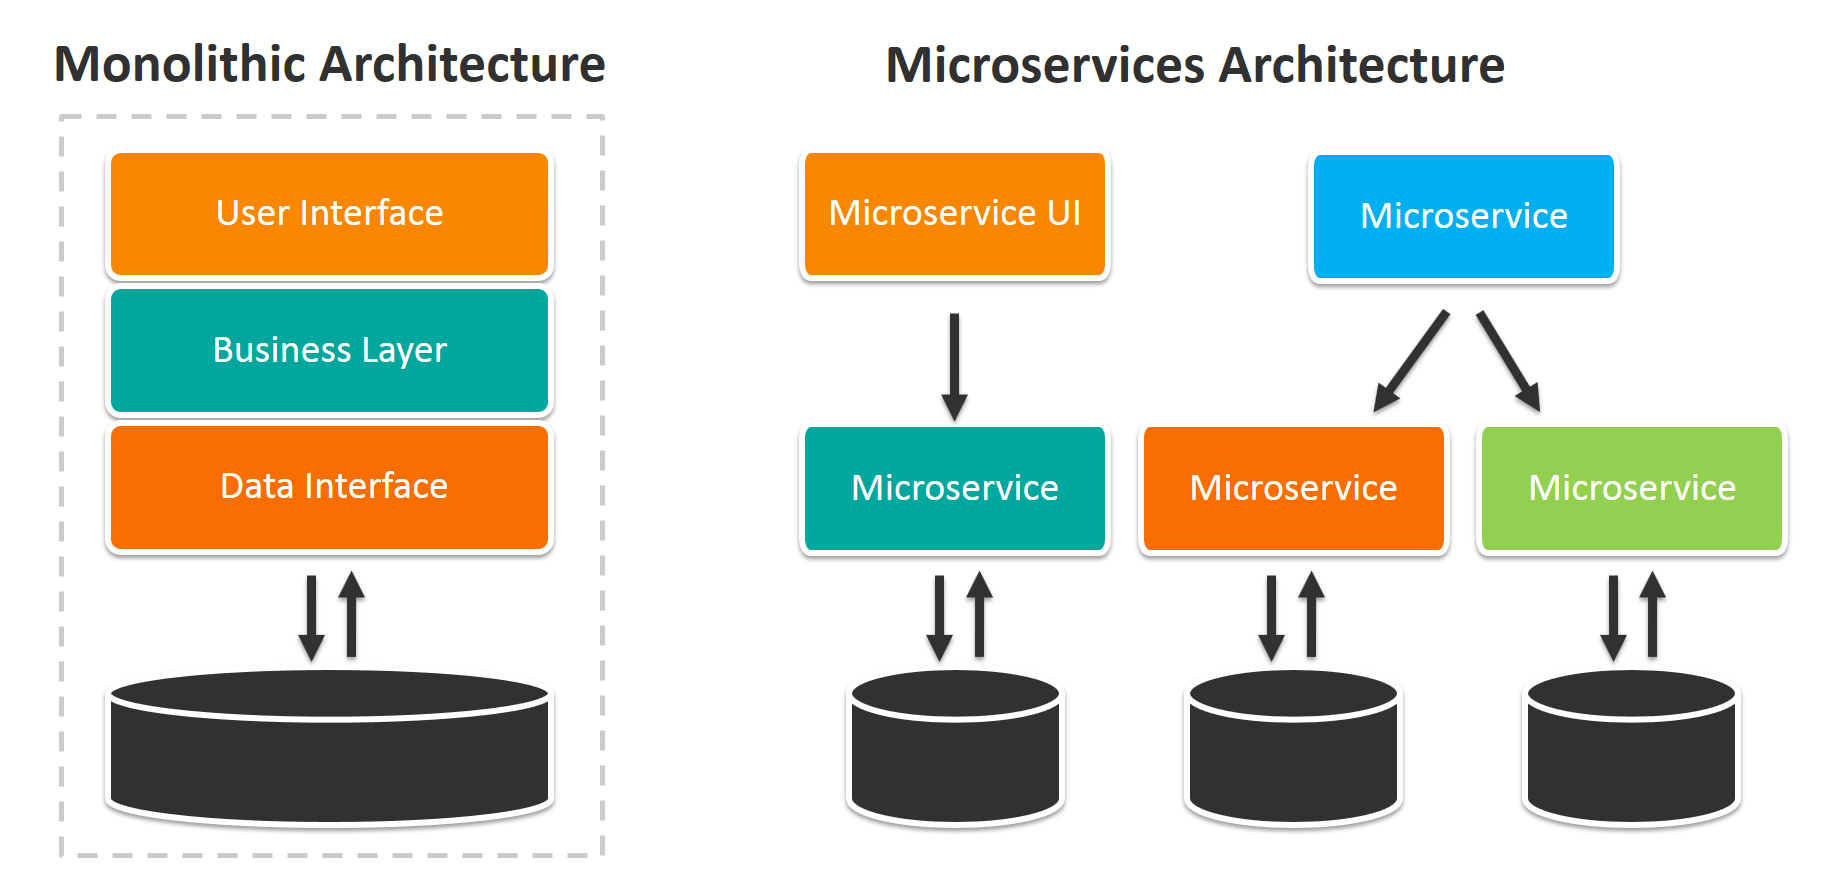
\includegraphics[width=10cm]{microservices-vs-monolithic.jpg}
	\centering
	\caption{Een monolithic architectuur naast een microservice architectuur. \textcite{Watts2018}}
\end{figure}
 De monolithic wordt  weergegeven in de linkerkant van de foto. Aan de rechterkant van de foto is een voorbeeld te zien van een microservice architectuur. Daar is duidelijk te zien dat elke microservice een eigen databank/datastore heeft. 
 Als er bij microservice A een probleem is, dan heeft dit niet meteen impact op de andere services. De communicatie tussen microservice A en de anderen zullen hier echter wel hinder ondervinden. Maar de andere microservices kunnen wel nog steeds onafhankelijk verder. 
 Hier ziet men dus duidelijk dat een microservice een klein component is van een groter geheel.
 Er is een mogelijkheid van de software om mee te groeien als het aantal gebruikers stijgt. De software moet nog even goed presteren bij 10 gebruikers als bij 2 000 gebruikers. Er wordt toegelicht hoe belangrijk API's zijn binnen een microservice architectuur. API's zijn een set van definities die ervoor zorgen dat deeltjes in een programma met elkaar kunnen communcieren. Een voordeel van API's is dat je niet moet  weten hoe de andere code werkt.

 Op figuur 2.2 ziet men dat de monolithic alle puntjes in een kader heeft. Dit staat symbool voor het grote geheel dat eigen is aan een monolithic. Alles zit samen in één grote doos. Maar bij microservices is dit niet zo, daar zit elk deeltje/requirement in een aparte doos, \textcite{Benetis2016a} . 
\begin{figure}[h!]
	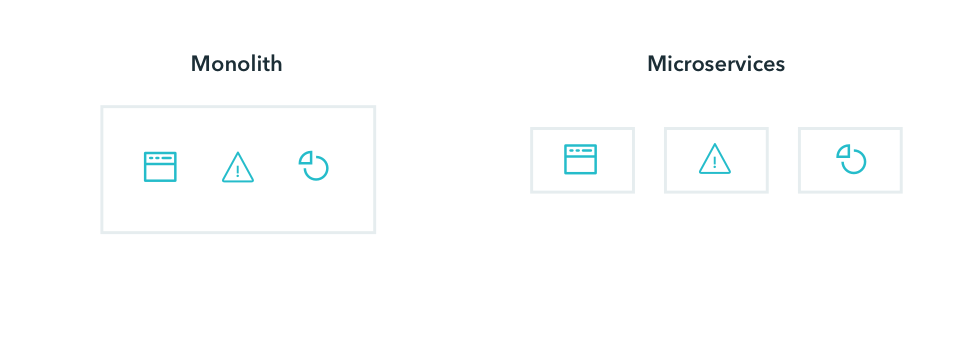
\includegraphics[width=10cm]{Mono_Micro.png}
	\centering
	\caption{Een monolithic vergeleken met een microservice. \textcite{Benetis2016a}}
\end{figure}


Een voorbeeld van een algemene architectuur is te zien op figuur 2.3.
\begin{figure}[h!]
	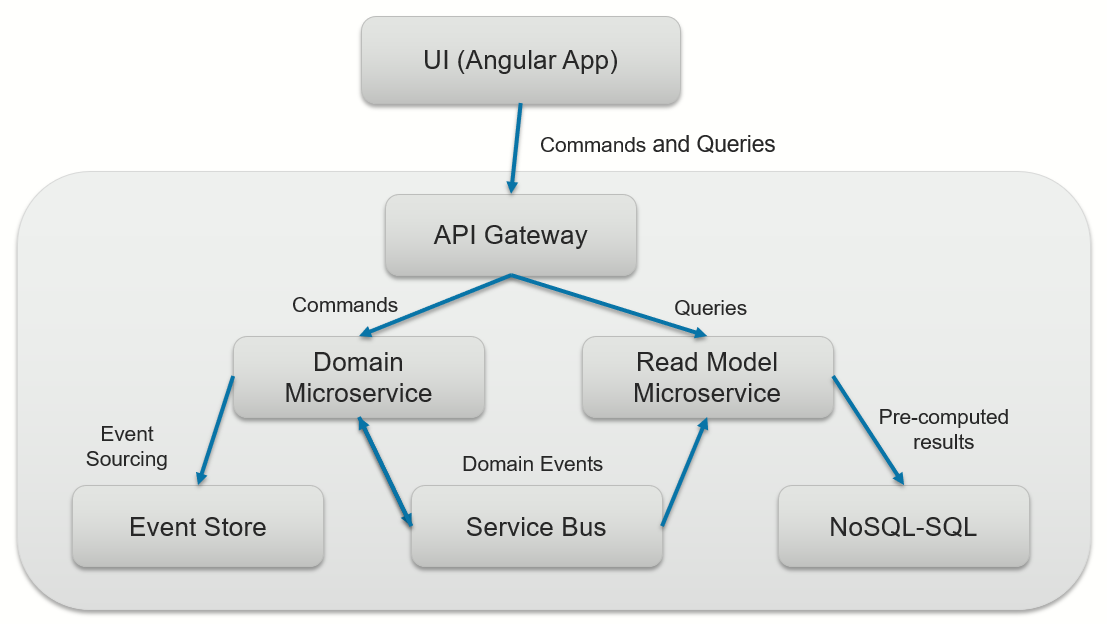
\includegraphics[width=10cm]{algArch.png}
	\centering
	\caption{Een algemene architectuur voor microservices. \textcite{Koukia2018}}
\end{figure}
Deze afbeelding zal later uitgelegd worden.


\subsection{Het belang van microservices}
Microservices zijn van belang wanneer de monolithic architectuur niet meer optimaal werkt. Microservices hebben nauwelijks invloed op het framework als er deeltjes bij gecodeerd worden. Ze kunnen sneller inspelen op de Agile analyse/ontwikkelsmethode. De analyse methode Agile werkt met periodieke opleveringen, die kunnen gaan van twee weken tot een maand. In die periode wordt er gewerkt aan een functionaliteit of een eis van de klant. 
Ervoor zorgen dat de software schaalbaar is, is een belangrijk punt en waar microsercies goed op inspelen.


Enkele andere redenen om microservices te gebruiken volgens \textcite{Koukia2018}, zijn ook:
\begin{itemize}
	\item Het is gemakkelijker om kleine services te onderhouden. Bij een monolithic is alles één groot geheel. Als daar een deeltje van moet worden aangepast, kan je verdwalen in het geheel. Dit is niet het geval bij microservices, want elke service is afgebakend met een functionaliteit. Bij het aanpassen van een service kan er duidelijk aangetoond worden waar een services begint en eindigt. 
	\item Een microservices kan onafhankelijk gedeployed worden. Eens een microservices klaar is voor gebruik, moet er naar niets anders gekeken worden. Bij het deeltje definitie  werd hier dieper op ingegaan.
	\item Gemakkelijker aan te passen aan nieuwe  technologie. Komt er een nieuwe  technologie uit die kan toegepast worden op een paar microservices, dan moeten enkel die microservices herschreven worden. Dit is anders bij een monolithic; als er een nieuwe  technologie is die kan toegepast worden op verschillende onderdelen van het geheel, moet de gehele architectuur herschreven worden.
	\item Het is eenvoudiger om te schalen. Schalen gebeurt door een microservice te dupliceren. Niet het gehele systeem moet geschaald worden, enkel de nodige microservices moeten gedupliceerd worden. Het dupliceren van een microservice wil zeggen, de microservice kopiëren en in een ander onderdeel gebruiken. Een microservice dat gedupliceerd kan worden, is dat van logging. 
	\item No single point of failure. Faalt er een microservices in het uitvoeren van zijn functionaliteit, dan heeft dit geen invloed op de andere services. Hier werd dieper op ingegaan in de definitie.
	\item Freedom of technology stack choices. Dit omvat dat elk team kan kiezen in  welke programmeertaal ze de microservices schrijven. Een team is verantwoordelijk voor één microservices. Ze zijn dus gespecialiseerd in die ene service. 
	\item De evolutie en de oplevering van business features is sneller. Dit komt door de onafhankelijkheid van de services. Er kan op hetzelfde moment aan verschillende services gewerkt worden zonder elkaar te beïnvloeden.
\end{itemize}


In de volgende stukken wordt er dieper ingegaan op de authenticatie en authorisatie, het verband met Agile en Devops, het debuggen binnen microservices en de bescherming van microservices.

\subsubsection{De verschillende manieren van bescherming}
'Microservices moeten een doel in de business vervullen. Naast dit, zorgen microservices er voor dat de bescherming eenvoudiger wordt.', \textcite{RDX2016}.

De term bescherming omvat het volgende: Ervoor zorgen dat hackers de applicatie niet kapot maken.
Hackers zijn mensen die inbreken op een applicatie.

Enkele tips om de bescherming van microservices aan te pakken, \textcite{Matteson2017}, \textcite{Silva2017}:
\begin{itemize}
	\item Zorg bij het ontwikkelen van microservices voor coderingsstandaarden die herbruikt kunnen worden. Door eenmaal een goede code te voorzien, wordt de kans op kwetsbaarheden en gaten in de bescherming kleiner.
	\item Ga na  welke schade er kan toegebracht worden aan een microservice als die zonder bescherming zou worden geüpload.
	\item Maak gebruik van toegangscontroles. Zorg ervoor dat er gewerkt wordt met leesrechten. Een microservice dat de aankooporders ophaalt, mag niet aan de verkooporders kunnen.
	\item Gebruik geen beveiligingsprincipes van externen maar implementeer deze liever in de code van de microservice.
	\item Zorg voor goede documentatie van elke microservice. Dit kan handig zijn bij het ontdekken van een zwak punt in de bescherming. De documentatie kan mogelijke problemen verduidelijken.
	\item Maak een API gateway. De bedoeling hiervan wordt verder nog uitgelegd.
	\item Zorg ervoor dat enkel de API gateway zichtbaar is en dat alle data onleesbaar verzonden wordt. Dit kan gebeuren aan de hand van SSL of TSL. Wat SSL is wordt verder in deze thesis uitgelegd. 
	\item Zorg voor garantie op data privacy. In Europa is de GDPR een  wetgeving die zegt wat er  wel en niet mag gebeuren met persoonlijke data. Daarom is het belangrijk dat er gebruik wordt gemaakt van een beveiligd protocol. Op elk level moet er gezorgd worden voor een correcte beveiliging van de gebruikers hun data. 
	\item Voor het encrypteren van data wordt er best gebruik gemaakt van al bestaande technologieën . 
	\item Zorg ervoor dat er geen denial of service kan gebeuren. Denail of service komt voor wanneer er heel veel requests naar de applicatie worden gestuurd, waardoor de applicatie faalt. Maak gebruik van throtteling. De term wordt na deze opsomming verder uitgelegd.
	\item Maak gebruik van Cross-site request forgery (CSRF) en Cross-origin resource sharing (CORS) filters. Cross-site request forgery is een poging tot hacken waarbij de eindgebruiker gedwongen wordt om acties te doen terwijl hij geauthenticeerd is. Cross-origin resource sharing laat toe dat er requests van een ander domein kunnen worden gemaakt. 
	\item De API gateway kan goed beschermd zijn maar zorg eveneens voor goede bescherming aan de code. Zorg ervoor dat er niks moet worden gerund als administrator, geef duidelijke namen en maak duidelijke afspraken. Enkel de nodige personen mogen de juiste permissies krijgen. 
\end{itemize}

\textcite{Troisi2019} geeft acht best practices over de bescherming van microservices. 
De best practices:
\begin{itemize}
	\item Het gebruik van OAuth voor gebruikers identificatie en wat de gebruiker kan. OAuth/OAuth2 is een protocol voor authorisatie. Het is een gemak om gebruik te maken van een protocol. Een protocol is een aantal regels om te communiceren tussen computers. 
	\item Gebruik bescherming in de diepte om een prioriteit toe te kennen aan service keys.  Dit kan verwoord worden als bescherming steken in verschillende lagen van een systeem. Er moet worden nagegaan  welke deeltjes het kwetsbaarst zijn en daar dan verschillende lagen van beveiliging op toe te passen. 
	Microservices maken het toepassen van deze methode eenvoudiger. omdat er gefocust kan worden op beveiliging. Het framework maakt het gemakkelijker om de verschillende lagen vast te stellen. Als hackers binnen zijn bij één van de microservices, zijn ze niet binnen in het volledige systeem. 
	\item Schrijf zelf geen krypto code. Er zijn genoeg open source alternatieven. Enkel bij heel uitzonderlijke redenen wordt een eigen krypto code geschreven. 
	\item Update je bescherming tijdig. Als er updates komen in de software van beveiliging, moeten die uitgevoerd worden. Het automatiseren van die updates kan veel  werk besparen achteraf. Dit wordt dan best gedaan bij het creëeren van microservices. Bescherming binnen software is niet langer meer een nice to have maar een must have. 
	\item Maak gebruik van een firewall met gecentraliseerde controle. Het biedt onder andere meer controle aan de gebruiker. 
	\item Maak gebruik van software om virussen te vinden.
	\item Monitor alles.
\end{itemize}

Throtteling, \textcite{Cavalcanti2018}, is een manier van bescherming die het volgende beschrijft: 'Throttling is a process used to control the usage of APIs by consumers during a given period.'. Het kan zijn dat de gebruiker heel veel requests stuurt naar de API gateway. Dit kan zorgen voor een bug door een oneidig aantal requests. Om dit te voorkomen kan er een limiet binnen een bepaalde periode opgelegd worden. Bijvoorbeeld als je je toegangscode drie maal fout hebt op je gsm, dan blokkeert die voor een bepaalde tijd. Het systeem dus zo ontwerpen dat het bestand is tegen fouten en falen. Met 'bestand zijn tegen' wordt bedoelt om ervoor te zorgen dat bij een bug of een fout waardoor deze goed wordt opgevangen zodat de gebruiker er geen last van heeft. 

Eén van de meer bekende manieren is de API gateway. De verantwoordelijkheden van een API gateway zijn de volgende, \textcite{Siraj2017}:
\begin{itemize}
	\item Het ontvangen van request van gebruikers.
	\item De requests doorsturen naar de correcte microservice.
	\item Het 'antwoord' van de microservice in ontvangst nemen en doorsturen naar de gebruiker.
\end{itemize}
Zoals te zien is op figuur 2.4, is een API gateway het toegangspunt. Om via de API gateway requests te kunnen maken, moet er eerst authenticatie en authorisatie toegepast worden. Meer uitleg hierover in de sectie over authenticatie en authorisatie.
\begin{figure}[h!]
	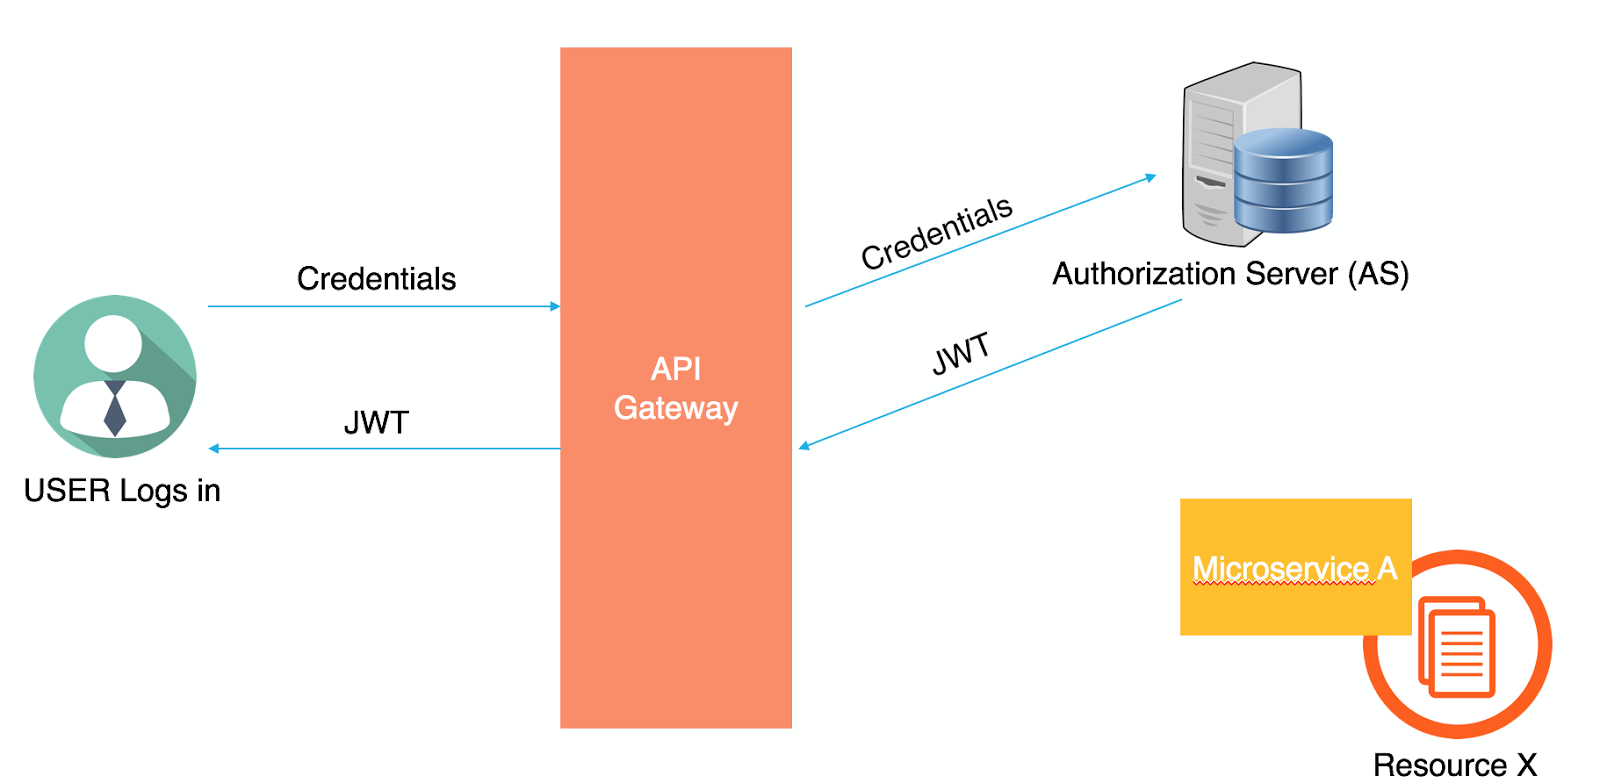
\includegraphics[width=10cm]{apiGateway_facadePattern.png}
	\centering
	\caption{Een voorstelling van API gateway. \textcite{Siraj2017}}
\end{figure}


\subsubsection{Authenticatie en authorisatie}
Een belangrijk aspect van microservices is de authenticatie en de authorisatie.  Het is een moeilijkheid om op een uniforme manier veiligheid, bescherming, authorisatie en authenticatie toe te passen op microservices, \textcite{Ayoub2018}. Authenticatie is het bevestigen van de identiteit van de gebruiker. Dit wordt doorgaans gedaan door middel van een gebruikersnaam en een wachtwoord. Authorisatie is wat je kan doen met een programma. Bijvoorbeeld een beheerder van een site kan meer dan een bezoeker. 
\begin{figure}[h!]
	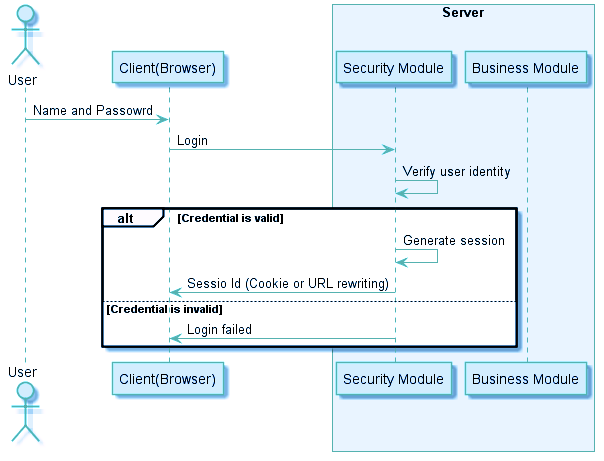
\includegraphics[width=10cm]{monolithic_auth.png}
	\centering
	\caption{Een diagram van authenticatie bij een monolithic. \textcite{Ayoub2018}}
\end{figure}
Zoals te zien is op bovenstaande afbeelding, figuur 2.5, wordt de authenticatie afgehandeld binnen het monlithic proces. Wanneer de gebruiker inlogt, wordt de beveiligingsmodule aangesproken. Deze kijkt of de gebruiker een bekende is, of er al gegevens in de databank zitten. Als het aanmelden gelukt is, wordt er een sessie gecreëerd. Een sessie wordt opgeslagen aan de hand van tokens. Tokens worden op je computer geplaatst door je browser. Het zijn kleine tekstbestanden. De sessie onthoudt wie je bent aan de hand van een ID. Dit zorgt er voor dat je je niet elke keer opnieuw moet aanmelden als je van pagina verandert.  Elke keer dat de bezoeker van de site iets doet, wordt de sessie ID samen gestuurd met de request. Een request is een aanvraag. Als het ID correct is,  weet de site dat de gebruiker ingelogd is. Bij elke aanvraag wordt de ID meegestuurd voor controle. Op die manier wordt de authenticatie bij een monolithic afgehandeld.
Wanneer er gekeken wordt om authenticatie toe te passen bij microservices, wordt het volgende aangehaald:
\begin{itemize}
	\item In elke microservice moet er authenticatie en authorisatie afgehandeld worden. Het beste wordt dit toegepast op een uniforme manier. Dan gaat men ervan uit dat er in elke microservices een stukje code komt dat hergebruikt wordt. Maar dit zorgt er voor dat elke microservice toch afhankelijk is. Bij het uitkomen van een nieuwe  versie, moet dit deeltje dan  weer geüpdate worden. Dit heeft invloed op de flexibiliteit van het framework.
	\item 'Single responsibility' zijn twee woorden die microservices mooi omschrijven. Een microservice omvat een stukje business logica. De algemene logica van authenticatie en authorisatie mag niet in een microservices gegoten worden. 
\end{itemize}
In het algemeen zijn authenticatie en authorisatie een complex onderdeel van microservices.
Er zijn vier oplossingen volgens \textcite{Ayoub2018}:
\begin{itemize}
	\item Distributed session manangement,
	\item client token,
	\item single sing-on, 
	\item client token with API gateway.
\end{itemize}
Distributed Session management is de eerste oplossing. Het managen van een sessie over microservices kan op verschillende manieren aan de hand van Sticky sessions. Dit houdt in dat alle requests van één gebruiker naar dezelfde server worden gestuurd waardoor men ervan kan uitgaan dat de gebruikte data van die specifieke gebruiker is. Of men kan dit toepassen via session replication. Dit houdt in dat alle instanties de sessie data synchronizeren. Deze manier van toepassen heeft als nadeel dat er veel overhead aanwezig zal zijn op het netwerk. Een andere methode is centralized session storage. Deze omvat dat bij het aanspreken van een microservice, deze de gebruikersdata ophaalt van op een gedeelde plaats. 
Een andere manier om authenticatie en authorizatie toe te passen, is via een client token. Een token wordt gebruikt om aan te tonen dat je echt de gebruiker bent. Een token wordt bijna altijd onleesbaar gemaakt. Het klinkt bijna hetzelfde als een sessie. Het verschil is dat een sessie op de server centraal wordt bijgehouden. Een token wordt bijgehouden door de user zelf.
Naast de Distributed session management en client token is er nog single sign-on. Na een enkele aanmelding kan de gebruiker alle microservices gebruiken binnen de applicatie. 
Een andere manier is een client token with API gateway. Deze manier is gebaseerd op de client token maar nu is er een API gateway toegevoegd aan het begin van een externe request. Dit zorgt ervoor dat het framework niet zichtbaar is voor de buitenwereld. 

Door de API Gateway to combineren met JSON  web Tokens is er meer mogelijkheid om te schalen,\textcite{Siraj2017}. 
\begin{enumerate}
	\item De gebruiker meldt zich aan.
	\item De API gateway stuurt de request door naar de server die instaat voor de auhtenticatie.
	\item Is de authenticatie goedgekeurd, wordt er een JWT token teruggestuurd naar de gebruiker. Meer uitleg over de JWT na dit proces.
	\item Bij de volgende request wordt de token automatisch meegestuurd met de request.
	\item Een andere server kijkt bij elke request naar de token om na te gaan of de gebruiker de juiste authorisatie heeft. 
\end{enumerate}
De token vervalt na een bepaalde tijd. Er kan gekozen worden om deze automatisch te laten verlengen. Hier wordt niet verder op ingegaan. 

De definitie van JSON  web Token, \textcite{Stecky-Efantis2016}: 'A JSON  web Token (JWT) is a JSON object that is defined in RFC 7519 as a safe way to represent a set of information between two parties. The token is composed of a header, a payload, and a signature.'. Het diagram te zien in figuur 2.6 is een schematische voorstelling van hoe een JWT token wordt gegeven aan een gebruiker.
\begin{figure}[h!]
	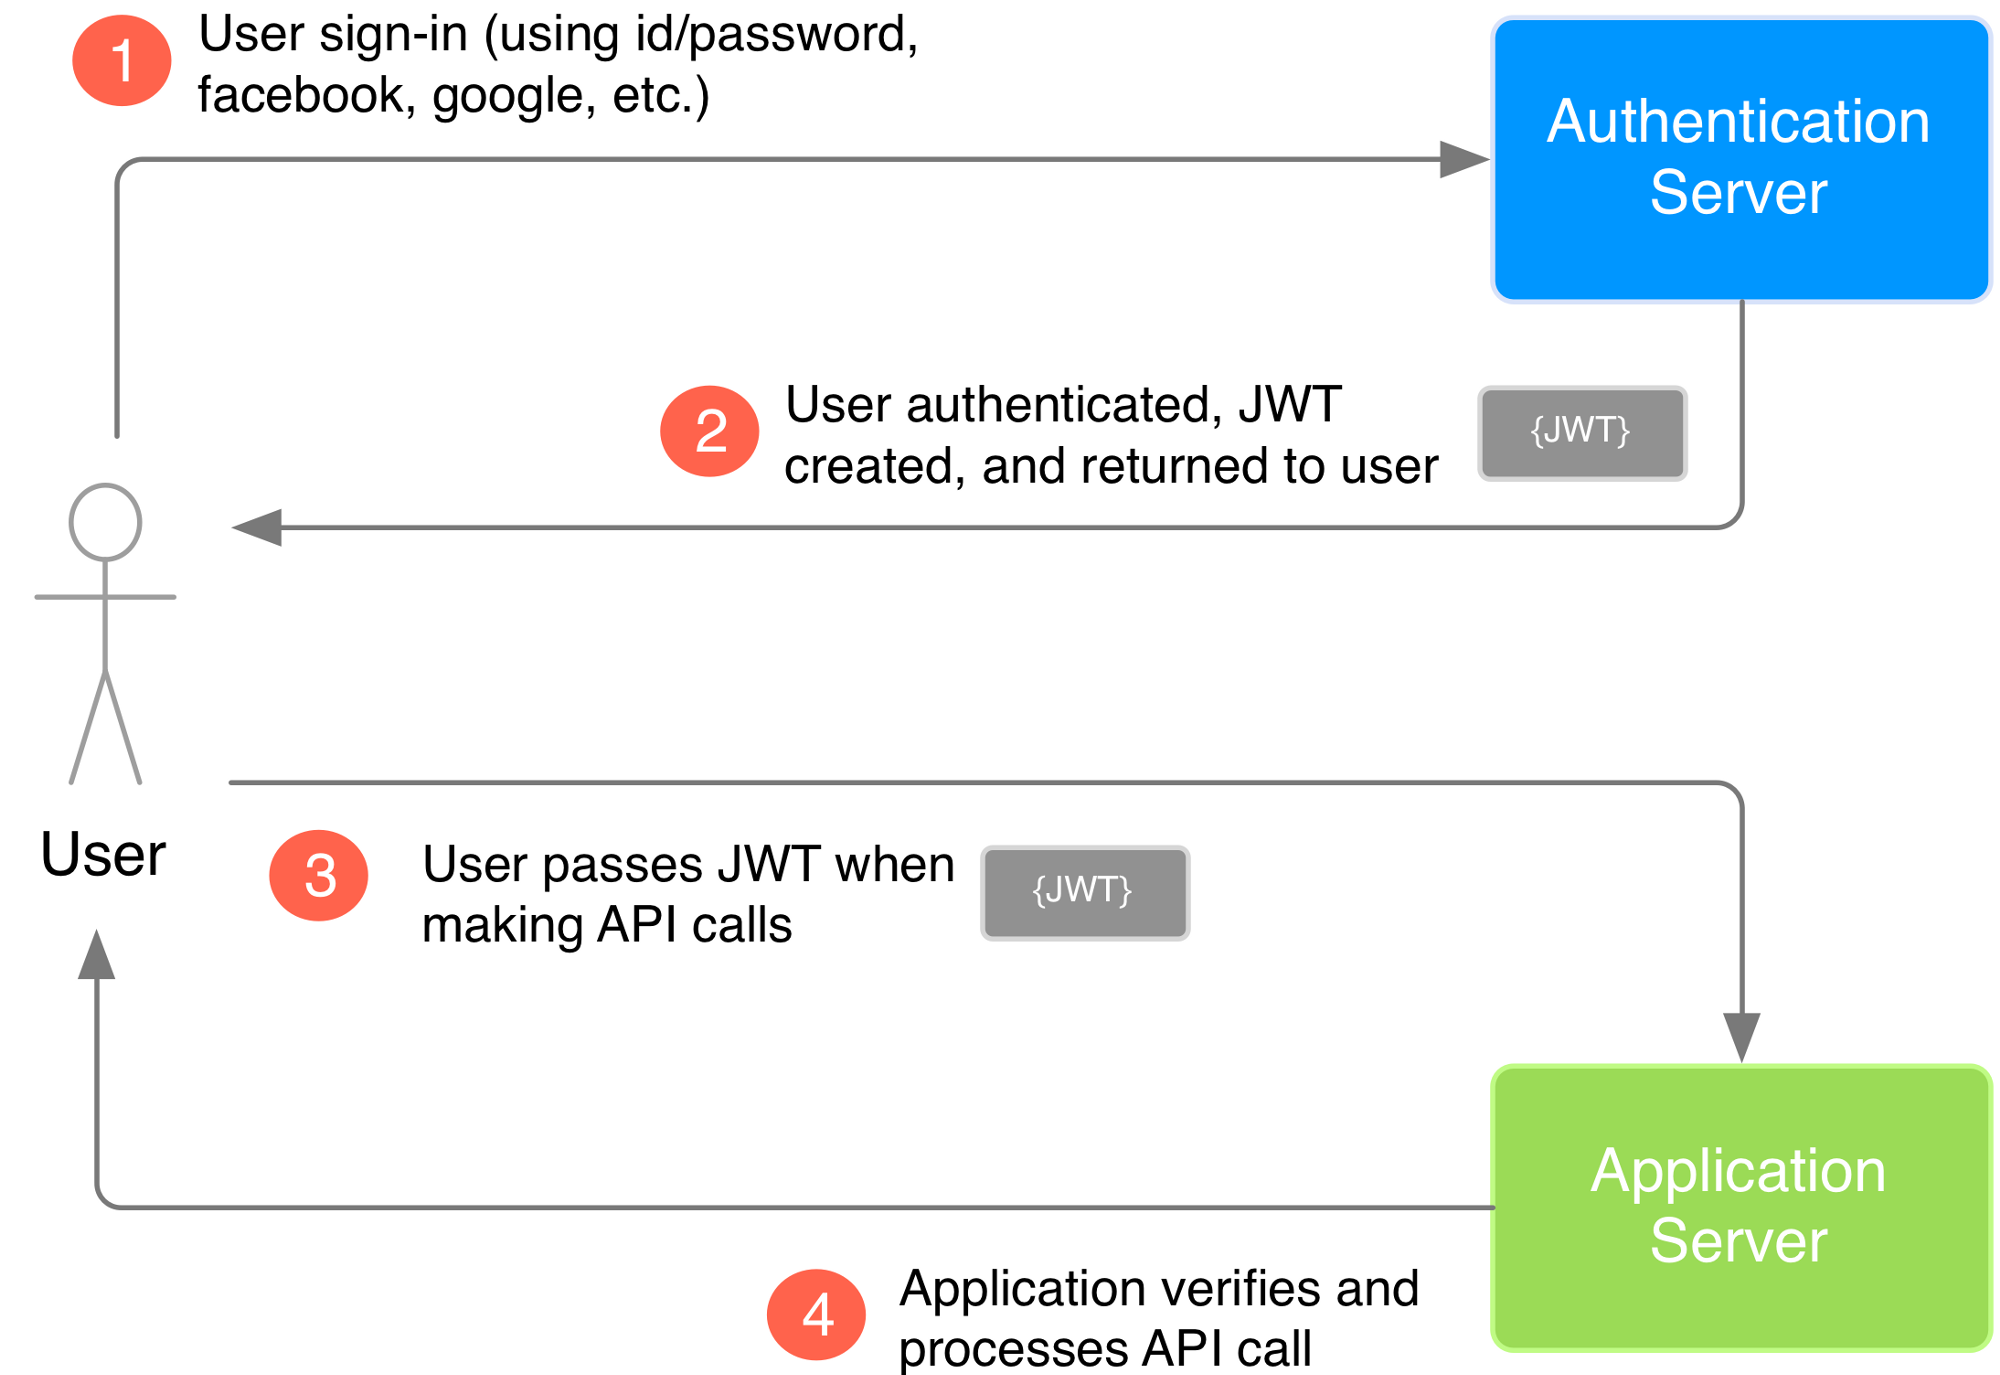
\includegraphics[width=10cm]{jwt.png}
	\centering
	\caption{Een schematische voorstelling van het geven van een JSON  web Token. \textcite{Stecky-Efantis2016}}
\end{figure}
Het proces gaat als volgt:
\begin{enumerate}
	\item Aanmelden op een platform. Bijvoorbeeld aanmelden op Facebook, Twitter, Instagram of Google.
	\item De authenticatie server stuurt een JWT terug.
	\item Bij het maken van requests wordt de token meegestuurd.
	\item De microservice kijkt dan of de gebruiker het recht heeft om deze microservice/functie te gebruiken.
\end{enumerate}


\subsubsection{Verband met Agile en DevOps}
Microservices komen uit dezelfde ideologie als Agile en DevOps. DevOps is een contaminatie  van development en operations. Bij deze methode ligt de nadruk op de samenwerking en communicatie tussen verschillende partijen. Hier zijn de partijen de software engineers en andere IT-specialisten. Deze ideologie omvat het volgende: het afbreken van een kleine, traag evoluerende architectuur of monolithic en deze in microservices steken.

DevOps heeft volgende definitie: 'DevOps is a methodology that enables developers and IT Ops to work closer together so they can deliver better quality software faster', \textcite{Morgan2019}. Met DevOps probeert men de productie zo goed mogelijk na te bootsen. Net zoals bij Agile, zorgt DevOps ervoor dat de software in kleinere delen wordt opgesplitst om opnieuw op kortere periodes deeltjes software op te leveren. Dit is iets waar microservices in terug te vinden zijn. Verschillende DevOps teams kunnen dus tegelijkertijd aan microservices  werken.

Enkele voordelen van de combinatie microservices en DevOps:
\begin{itemize}
	\item Meer opleveringen van software op kortere periodes.
	\item Betere kwaliteit van de code.
	\item Software kan hergebruikt worden.
	\item Een hoger level van automatisatie.
\end{itemize}

Microservices en DevOps vullen elkaar aan op volgende vlakken, \textcite{Mulesoft2019}:
\begin{itemize}
	\item Deployability: Microservices bemoedigen het gebruik van Agile omdat het eenvoudiger is om periodiek op te leveren. 
	\item Reliability: Een fout binnen een microservice, heeft enkel effect op die microservice. 
	\item Availability: Het opleveren van nieuwe  deeltjes neemt niet veel tijd in beslag. De gehele applicatie zal niet lang offline zijn.
\end{itemize}




\subsubsection{Het monitoren van microservices}
Logs zijn records binnen een databank die weggeschreven worden terwijl de applicatie draait. Metrics zijn numerieke waarden die kunnen geanalyseerd worden. Metrics zijn terug te vinden op volgende niveau's van een applicatie, \textcite{Wasson2018}:
\begin{itemize}
	\item Node-level: Dit bevat de gegevens van de CPU, het geheugen, netwerk en de harde schijf. 
	\item Applicatie: Hier kunnen metrics bijgehouden worden om het gedrag van de service te begrijpen. Gegevens die bijgehouden kunnen worden zijn het aantal HTTP requests, de vertraging en de lengte van een bericht.
	\item Dependent service: Bij interactie met een externe service kijken hoe lang deze duurt om te reageren. 
\end{itemize}


Het monitoren of loggen van microservices houdt in dat er bijgehoduen wordt hoe een microservice zich gedraagt. Er wordt bijvoorbeeld bijgehouden hoe snel de data wordt opgehaald uit de databank. Monitoren vomt dus een belagnrijk onderdeel bij het vinden van problemen. \textcite{Ananthasubramanian2018}.


De verschillende tools om te debuggen, \textcite{Swersky2019}:
\begin{itemize}
	\item Logging frameworks: Het is een open-source oplossing. Er zijn verschillende opties; bij het kiezen wordt er best rekening gehouden met volgende puntjes:
		\begin{itemize}
			\item De netheid van de code. Is de logging code gemakkelijk te lezen?
			\item Wordt de performance beïnvloedt?
			\item Is het framework voor logging al gekend bij het team?
		\end{itemize}
	\item Logging databases: Log data wordt gebruikt voor het capturen van events. Logs worden nooit aangepast en worden gesorteerd op datum en tijd. 
\end{itemize}



Bij microservices wordt elke microservice gelogd. Bij een fout moet er gekeken worden naar alle betrokken microservices. Er moet gekeken worden naar alle logs van de services. Om logging toe te passen, wordt er aangeraden om libraries te gebruiken. Enkele best practices, \textcite{Melendez2018}, \textcite{Eyee2018}, \textcite{Timms2018}:
\begin{itemize}
	\item Probeer te vermijden dat logs in bestanden worden opgeslagen. Logs zijn streams van een flow. Het geeft  weer wat er precies gebeurt is in een flow.
	\item Microservices moeten niet  weten waar de logs naar toe gaan. Zo kan de bestemming van het  wegschrijven van de logs veranderd worden zonder dat elke microservice ervoor aangepast moet worden.
	\item De logging moet werken voor alle verschillende codeertalen. Er moet niets worden aangepast bij de configuratie files van het logging systeem.
	\item Geef elke request een uniek ID. Zo kan de request snel teruggevonden worden bij falen. Of bij het zien van een fout kan er snel achterhaald worden  welke request er in fout is gegaan. 
	\item Laat het antwoord een uniek ID meesturen. Als de gebruiker dan een fout krijgt, kan er achterhaald worden waar de teruggestuurde fout vandaan komt. De administrators kunnen dan de details van de fout bekijken.
	\item Een oplossing is om alle logs  weg te schrijven naar een centrale databank. Zo kan het hele pad van de fout snel en eenvoudig teruggevonden worden. Het duurt langer om verschillende fouten aan elkaar te linken als de logs in de datastore van de microservice worden opgeslagen. Bij het opslaan op één plaats worden fouten sneller aan elkaar gelinkt. Het  wegschrijven naar een plaats is tegen het principe van microservices. Binnen die enkele database met alle logs kan er gezocht worden op fout, microservice, tijdstip, ...  het volgen van een gebruiker zijn traject binnen de applicatie is eenvoudiger. Bij een fout kan er gekeken worden naar de acties die er op voorhand zijn gemaakt. 
	\item Zorg voor structuur in de log data. Gebruik een algemene format zoals JSON of XML om een structuur te creëeren in de logs. 
	\item Geef iedere request een context.  De oorzaak van de fout kennen, is belangrijk om ervoor te zorgen dat de fout zich niet zal herhalen. Volgende velden zouden zeker in de log terug te moeten vinden zijn:
		\begin{itemize}
			\item Dag en tijd.
			\item Stack errors.
			\item De naam van de service, om de logs te linken aan microservices.
			\item In  welke functie de fout is ontstaan.
			\item De naam van de externe service waar er interactie mee is geweest.
			\item Het IP adres van de server en van de gebruiker zijn requests. 
			\item De browser waaruit de gebruiker de request stuurde.
			\item De HTTP code om later alerts te creëren. 
		\end{itemize}
	\item Overweeg om de logs naar een lokale databank  weg te schrijven. Elke oplossing heeft zijn voor- en nadelen. Het  wegschrijven over HTTP naar de cloud kan zorgen voor meer verkeer op het netwerk. De bandbreedte kan bij belangrijke microservices verminderd worden. 
	\item In het begin wordt er best veel gelogd. Later kan beslist worden om enkele parameters niet meer te loggen.
\end{itemize}



\subsection{De voordelen en nadelen van microserivces}
Het gebruik van microservices zorgt ervoor dat de architectuur flexibeler wordt.  Dankzij microservices is het hermodeleren, implementeren van nieuwe  technologieën, ... eenvoudiger.
Kleinere deeltjes zijn gemakkelijker te documenteren. Ook de snelheid van microservices zijn een groot pluspunt. Microservices reageren sneller  omdat zo kleine, onafhankelijke services zijn. Ze moeten geen onnodige stappen maken om de  wens van de klant te vervullen. 

\textcite{Watts2018} geeft nog andere voordelen van een microservice. Een developer is onafhankelijk, ze moeten niet wachten een andere developer. 

Het scalen van een microservice is veel eenvoudiger. Omdat dat microservices minder resources nodig hebben dan een volledige monolithic. Resources zijn hulpbronnen onder andere protocollen, programmeerstandaarden... 

Binnen een monolithic zijn deeltjes afhankelijk van elkaar om goed te kunnen functioneren. Een ander voordeel: bij het falen van een microservices zal de ander geen last ondervinden. 

\textcite{Benetis2016} geeft aan dat microservices sneller en gemakkelijker te deployen zijn. Dit is een gevolg van een ander voordeel: microservices zijn onafhankelijk. Ze kunnen elk op hun eigen tempo gedeployed worden.

Een eerste nadeel is dat de scope gedetailleerder moet zijn omdat het project ingedeeld is in kleinere requirements. Als gevolg daarop zijn de teams kleiner en een teamlid kan niet zomaar vervangen worden omdat elk team een bepaalde specialisatie heeft.

\textcite{Koukia2018} drukt ons op het feit dat het onderhouden van microservices vraagt veel werk. Het is een nieuwe technologie en het team moet up to date blijven over die technologie. Dit is een van de redenen waarom sommigen bij een monolithic blijven. De complexiteit binnen monolithic is gekend. De developers zijn gewoon om met die complexiteit te werken en er fouten uit te halen. Daarom lijkt de chaos bij microservices soms groter dan bij een monolithic.

\section{Microservices integration patterns}
Hierboven werd uitgelegd wat microservices zijn. Het zijn kleine, onafhankelijke services die aan business requirements voldoen. Maar die moeten met elkaar kunnen communiceren, taken uitvoeren, data updaten en elkaar kunnen raadplegen. Om ze met elkaar te laten communiceren, moeten ze op een gestructureerde manier geintegreerd worden in de applicatie. Gestructureerd integreren kan a.d.h.v. onderstaande patterns:
\begin{itemize}
	\item Anti-patterns
	\item Communicatie tussen de microservices
	\item Data integration
	\item Extract, transform en load (ETL)	
\end{itemize}

In het derde hoofdstuk zal één of meerdere van de bovenstaande patterns theoretisch toegepast worden op het order-to-cash proces. Het order-to-cash proces zal verder uitgelegd worden in deel 2.3.
\subsection{Anti-patterns}
Een anti-patterns is het implementeren van microservices op een ongestructureerde manier zonder grondig onderzoek te doen. 
Anti-patterns ontstaan bij een ongeplande overschakeling naar microservices.  Anti-patterns komen vaker voor dan een gestructureerde microservice architectuur omdat ongepland en gewoon ergens aan beginnen eenvoudiger is dan alles plannen en voorbereiden. Er moet grondig onderzoek gedaan worden naar de verschillende 'microservice integration patterns'. Op welke manier kan de applicatie gestructureerd naar een microservice architectuur verandert worden?
De meeste mensen hebben niet door dat ze een anti-pattern aan het maken zijn. . 

Er zullen drie anti-patterns besproken worden die kunnen helpen bij het achterhalen ervan. Volgende zullen besproken worden, \textcite{Monson2019}:
\begin{itemize}
	\item Break the piggy bank
	\item Everything micro
	\item We are Agile: The Frankenstein
\end{itemize}
\subsubsection{Break the piggy bank}
Op een break the piggy bank structuur lijkt de applicatie wat op een spaarvarken. Om van een monlithic applicatie naar een microservice applicatie te gaan, moet de applicatie uit elkaar gehaald worden en opgedeeld worden in kleine delen.  De kleine delen worden omgezet naar microservices. 
In het begin van de verandering naar microservices zal de complexiteit verminderen. Maar  verder in het proces wordt het enkel complexer door de ongestructureerde overgang.
De applicatie is opgedeeld in onderdelen en die onderdelen zijn omgezet in microservices. Bij het samenvoegen van de microservices tot een architectuur, is het mogelijk dat de applicatie een mini-monolithic wordt. Dit komt voor wanneer de services niet opgedeeld worden op basis van functionaliteit en willekeurig worden samengevoegd zonder op voorhand na te denken.
Dit anti-pattern is het populairst wanneer een monolithic applictie niet meer houdbaar is. Dit pattern kan goed gebruikt worden als het in combinatie met een ander integration pattern wordt gebruikt.
De figuur 2.7, die dit anti-pattern illustreerd, is terug te vinden op pagina 31.
\begin{figure}[h!]
	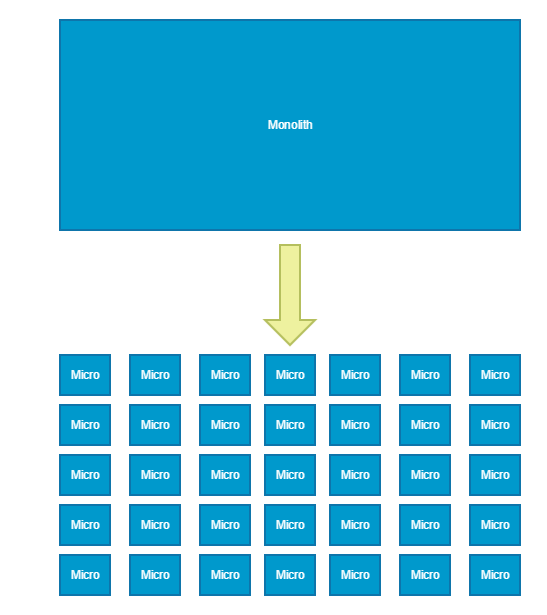
\includegraphics[width=10cm]{breakthepiggybank.png}
	\centering
	\caption{Break the piggy bank, van monolithic naar microservices via anti-pattern \textcite{Monson2019}}
\end{figure}

\subsubsection{Everyting micro}
Alles in de applicatie wordt omgezet naar microservices, behalve de databank. De verschillende microservices moeten de data uit een gemeenschappelijke databank opvragen. Deze wordt dan snel de 'bottleneck' in de applicatie. De term 'bottleneck' wordt gebruikt wanneer een plaats is binnen de applicatie waar alle delen vertraagd worden. Alle aanvragen komen binnen maar er kunnen maar enkele verwerkt worden.
Om de data van de databank op te halen moet er aan 'access control' uitgevoerd worden. Niet alle microservices kunnen tegelijkertijd hun data opvragen en ontvangen.
Dit moet op een gecontroleerde manier anders is er kans op 'deadlock'. Deadlock komt voor wanneer twee of meerdere services data van de databank willen halen. 
De datastructuur blijft in feite monolithic.
Eerst lijkt dit niet zo een groot probleem. Naast Naast een verhoogd risicoop vertragingen, komt dit anti-pattern ook met een extra uitdaging: de verandering van de databankschemas bijhouden. Omdat er maar één databank gebruikt wordt, moet elke verandering van elke microservices genoteerd worden. Naast die uitdaging, moet bij een verandering in de productie databank, de volledige applicatie opnieuw gedeployed worden. Een productie databank is de databank die live gebruikt wordt door klanten. Een voorbeel van een productie databank: de databank waarmee je communiceert als je op Zalando iets besteld. Een alternatief voor dit is terug te vinden in 'Data integration'.
Figuur 2.8 illustreert hoe 'everything micro' er kan uitzien. Dit is terug te vindne op pagina 32.
\begin{figure}[h!]
	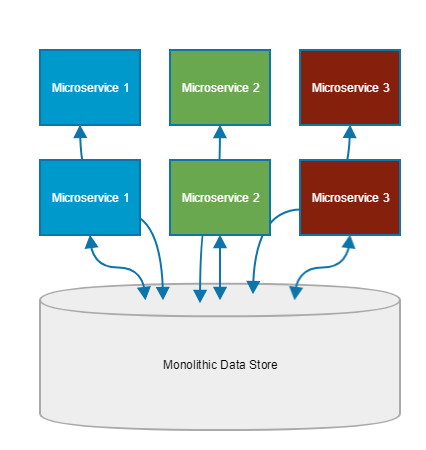
\includegraphics[width=10cm]{everythingmicro.png}
	\centering
	\caption{Everyhting micro, anti-pattern met een monolithic databank. \textcite{Monson2019}}
\end{figure}

\subsubsection{We are Agile: The Frankenstein}
Dit anti-pattern ontstaat vaak door de overschakeling van watervalanalyse naar de Agile methodologie. Bij watervalanalyse wordt er één groot plan opgesteld voor een project. Dat plan wordt uitgevoerd met de hoop dat er geen veranderingen worden doorgevoerd in het project. 
Door de simpliciteit van de omschakeling wordt soms gedacht dat er geen voorbereiding nodig is. Dat alles duidelijk zal worden eens het probleem zich echt voordoet. De meeste teams gaan van de waterval methode naar een combinatie van Agile en waterval. 
Het gevolg van een ongestructureerde planning zijn delen die los van elkaar zijn geprogrammeerd en die niet kunnen samenwerken. Ze worden aan elkaar 'genaaid' om samen te werken. Net zoals Frankenstein aan elkaar is genaaid met verschillende onderdelen. De samengevoegde onderdelen moeten de databank delen. Telkens er een nieuwe functionaliteit moet toegevoegd worden, wordt de architectuur complexer en moeilijker om te deployen. 
Omdat de architectuur een ongestructureerd samenhang is van losse onderdelen, kan de applicatie op lange termijn transacties doen waarvoor die niet geprogrammeerd is. De applicatie loopt het gevaar uit elkaar te vallen.
De mogelijkheid bestaat dat de applicatie gewoon uit elkaar valt door de slechte architectuur en de chaos die er is. 
De figuur 2.9 geeft een duidelijker beeld van deze methode, de afbeelding is terug te vinden op pagina 33.
\begin{figure}[h!]
	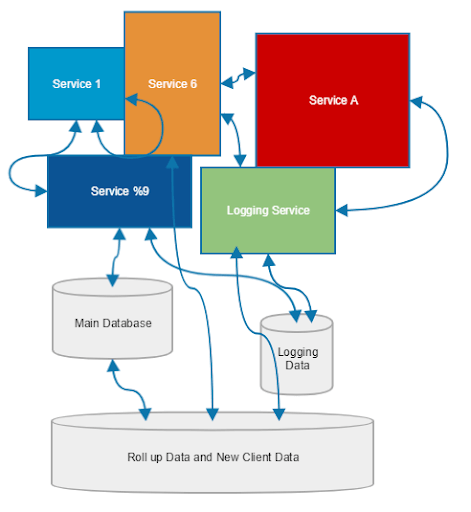
\includegraphics[width=10cm]{frankenstein.png}
	\centering
	\caption{The Frankenstein, anti-pattern waarbij de microservices bij elkaar zijn gevoegd zonder samenhang. \textcite{Monson2019}}
\end{figure}



\subsection{Communicatie tussen de microservices}
Er zijn verschillende manieren om microservices te laten communiceren met elkaar. 
De microservices kunnen elke microservice kennen die het nodig heeft. Maar dit maakt de gehele architectuur enkel maar complexer. Zoals in afbeelding 2.10 te zien is (pagina 33), zorgt deze manier van communicatie voor een chaotische architectuur.
\begin{figure}[h!]
	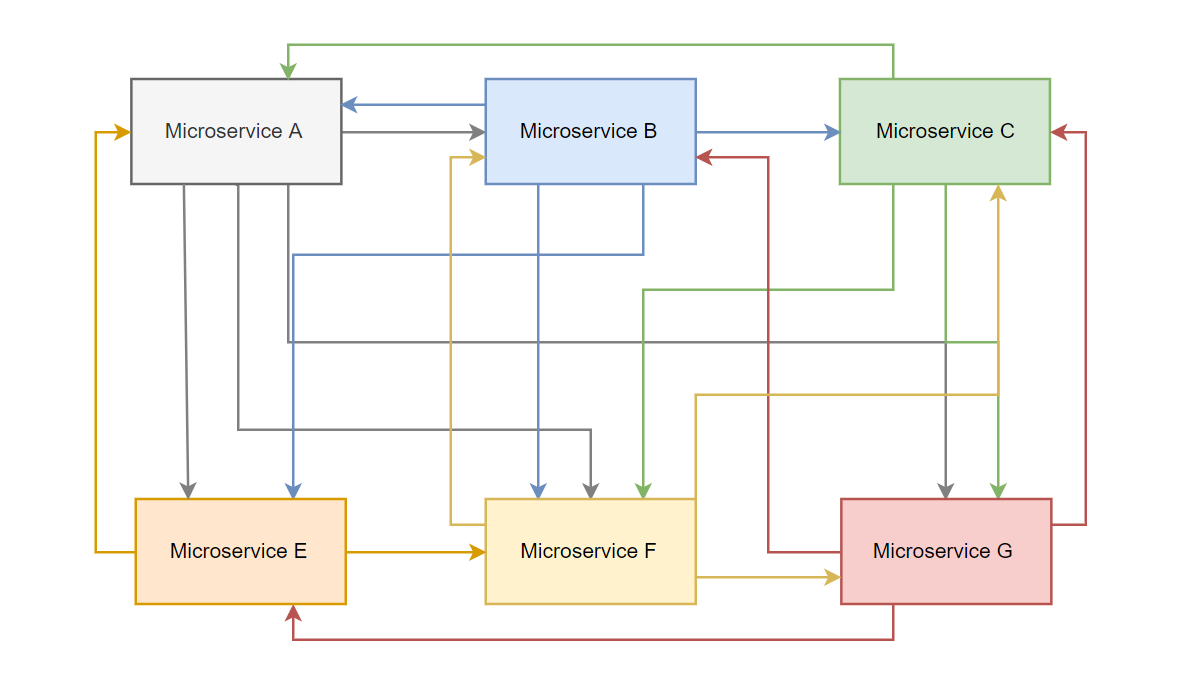
\includegraphics[width=10cm]{chaos.PNG}
	\centering
	\caption{Een architectuur waarbij de microservices elkaar direct kennen om informatie met elkaar te delen.}
\end{figure}

Afbeelding 2.10 illustreert dat de microservices niet meer onafhankelijk zijn en vormen een mini-monolithic. Om ervoor te zorgen dat de microservices onafhankelijk blijven, kan er messaging toegepast worden, \textcite{Solance2018}. Messaging is een manier van communiceren, om business entiteiten up te daten, waarbij een 'message broker' gebruikt wordt. Een 'message broker' is de logica die de berichten van een microservice naar een andere stuurt zonder dat ze elkaar moeten kennen. Het meest gekende patroon hiervoor is publish-subscribe pattern. Deze wordt weergegeven in afbeelding 2.11.
\begin{figure}[h!]
	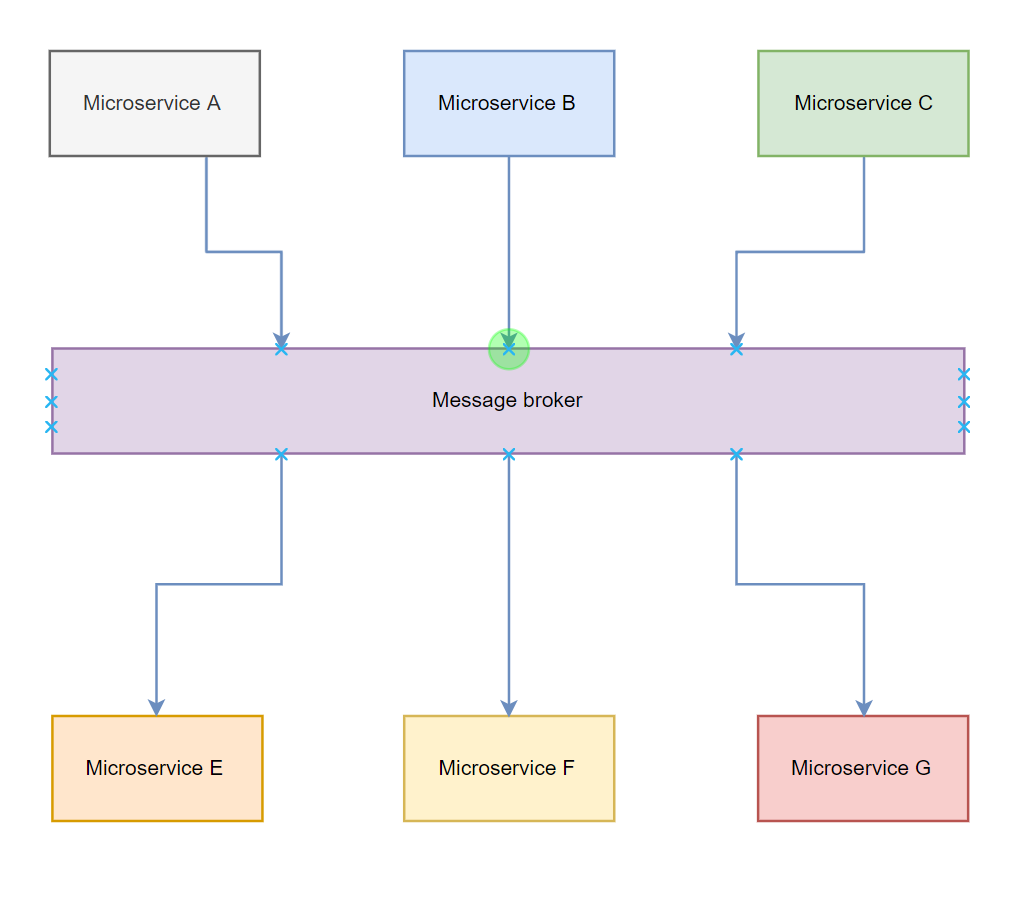
\includegraphics[width=10cm]{messaging.PNG}
	\centering
	\caption{Een architectuur waarbij een message broker als communicatiemiddel wordt gebruikt.}
\end{figure}
In de 'message broker' heeft elke microservices zijn queue. De queue is een wachtrij waar berichten worden opgeslaan. De berichten worden verwijderd van de queue eens ze gelezen en opgehaald worden. 
Een microservice stuurt een bericht naar de 'message broker' en moet zich verder niks van het bericht aantrekken. De 'message broker' zorgt ervoor dat het bericht bij de juiste microservice(s) wordt afgeleverd. De uiteinden kennen elkaar niet en volledig onafhankelijk van elkaar communiceren.

\subsection{Data integration}
Data integration wordt door \textcite{Aradhye2018} en \textcite{Kumar2018} uitgelegd. Data integration is een manier om de data van microservices weg te schrijven, op te halen, op te slaan in een databank.
Een opvallende eigenschap aan een monolithic architectuur is de centrale databank. Bij de overgang wordt de databank regelmatig uit beeld gelaten, nochtans is het ook de databank die echter een grote verandering moet ondergaan. Maar de structuur waarmee er met de data wordt gewerkt, verandert. 
De monolithic databank kan nog gebruikt wordt bij een microservice architectuur, maar  dat brengt veel problemen en obstakels met zich mee. Volgende zijn enkele voorbeelden:
\begin{itemize}
	\item De microservices zijn afhankelijk van dezelfde databank en dus van elkaar. Als ze meerdere microservices de databank nodig hebben, moeten ze hun beurt afwachten.
	\item Microservices onafhankelijk deployen, is onmogelijk. Een aanpassing heeft invloed op de databank en elke microservice kent de databank. 
	\item Een microservice scalen wordt een moeilijke opgave omdat die vasthangt aan de centrale databank. 
	\item Omdat alle data in één databank wordt bijgehouden, worden de tabellen gigantisch groot en op termijn onhoudbaar en slordig. 
\end{itemize}

Elke microservices heeft zijn eigen databank met data betreffende hun functionaliteit. Hieronder kunnen enkele voorbeelden teruggevonden worden over de voordelen van een microservice met een eigen databank:
\begin{itemize}
	\item De databank bevat enkel de relevante data.
	\item Elke microservices kan apart gedeployed worden. 
	\item Een microservices heeft geen rechtstreekse toegang tot de databank van een andere microservices. 
\end{itemize}

Sommige microservices hebben data van andere microservices nodig omdat hun databank de gewenste gegevens niet kan leveren. De data wordt dan opgevraagd aan de databank waar de gewenste data staat via een de microservice zelf. Dit wordt geillustreerd in afbeelding 2.12, terug te vinden op pagina 34.
\begin{figure}[h!]
	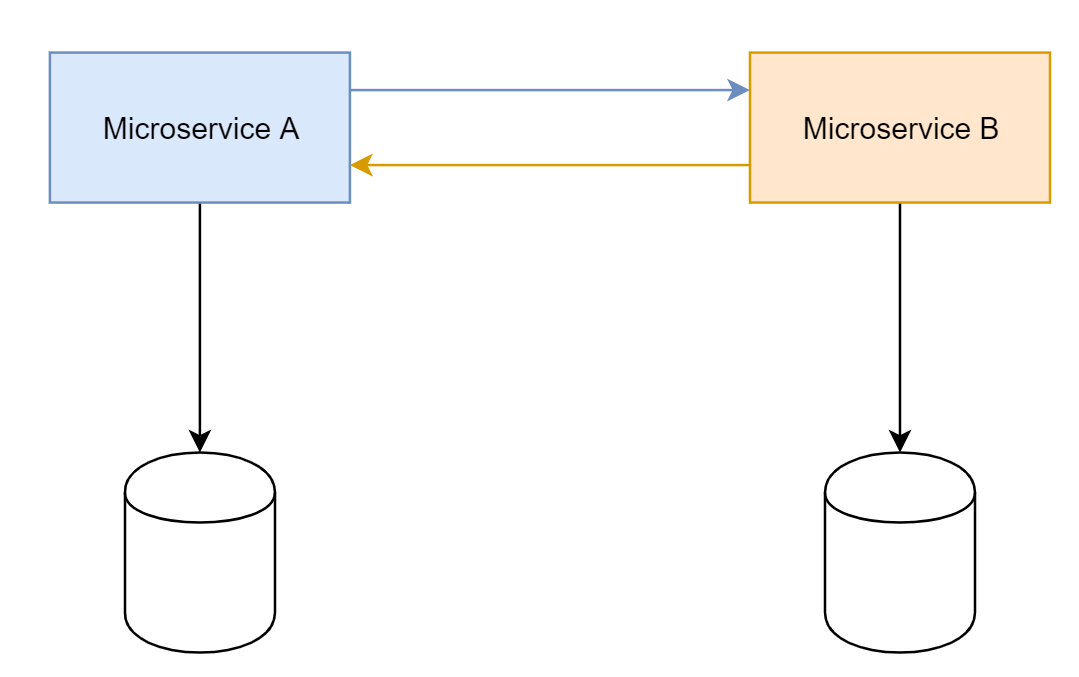
\includegraphics[width=10cm]{db.PNG}
	\centering
	\caption{Hoe een microservice de databank van een andere microservice aanspreekt.}
\end{figure}
 
De manier waarop licroservices gegeven uitwisselen uit elkaars databank werd beschreven in het vorige deel over 'communicatie tussen de microservices'.
 
Eens de volledige communicatie is uitgedacht, moet er een databank gekozen worden, die past bij de micoservices. Het kan zijn dat voor de ene microservice een SQL-databank beter past en voor de ander een NOSQL-databank. SQL en NOSQL zijn soorten databanken. Het verschil tussen de twee is de manier van data opslaan en de manier hoe data wordt opgehaald. Maar dit aantonen is niet het doel van deze scriptie.
 
\subsection{Extract, transform en load (ETL)}
De uitleg over ETL is gebaseerd op artikels van \textcite{Loshin2019}, \textcite{Alley2018}, \textcite{Stich2019}, \textcite{Guru2019} en \textcite{Naveen2016}.

ETL wordt gebruikt  om data te verzamelen, te transformeren en in een andere databank te steken. De data wordt geanalyseerd om het bedrijf een beter beeld te geven van de real-time gebeurtenissen bij bijvoorbeeld marketing. Ze kunnen te weten komen wat het meest verkocht wordt om 12 uur 's middags. 
ETL bestaat uit drie stappen.
De eerste stap is 'extraction', de data ophalen. De verzamelde data komt niet van één databank. Ze wordt opgehaald uit verschillende bronnen. Die bronnen zijn databanken die online informatie bevatten over het gedrag van die klant. Belangrijk is het verzamelen van de data mag de werking van de originele databank niet beïnvloeden.
Na het verzamelen van de data, wordt die getransformeerd en gefilterd om enkel de nodige data te gebruiken. Er wordt meer data verzameld dan nodig, dus is het belangrijk dat data gefilterd wordt.
Die data wordt ingelanden in een datawarehouse. Een datawarehouse is een databank waar men data analyseert en logica gebruikt. De business legt op welke analyse er moet gebeuren. De uitkomst van deze analyse kan gebruikt worden binnen het bedrijf of kan gebruikt worden voor artificiële intelligentie.  

\begin{figure}[h!]
	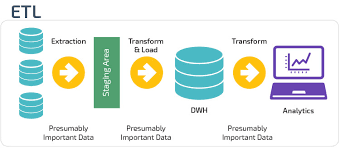
\includegraphics[width=10cm]{etl.PNG}
	\centering
	\caption{Hoe het ETL proces eruit ziet. \textcite{Panolapy2019}}
\end{figure}


\section{Order-to-cash proces in SAP}
\subsection{Definitie}
Het OTC proces is het proces dat begint bij het order plaatsen en eindigt bij het betalen van de facturatie en de analyse van de gegevens verzameld tijdens het proces. Deze wordt gebruikt om het verkopen van producten goed te laten verlopen binnen het bedrijf.

Order management is de eerste stap in het proces. Dit begint wanneer de klant een order plaatst. Bijvoorbeeld: ik besteld schoenen op Zalando. Dit deeltje van het proces moet geautomatiseerd zijn om het proces zo snel mogelijk te laten verlopen. Als dit deel van het proces niet goed opgezet  is, dan kan het snel slecht gaan. Bijvoorbeelden: orders zitten dubbel in de databank.

Na het plaatsen van een order, wordt de klant gecontroleerd. Hierna volgt Credit management. Dit moet ervoor zorgen dat er minder problemen zijn op het einde van het proces. Credit management houdt in dat men kijkt naar hoe het betalingsgedrag van de klant is geweest. Zijn er nog openstaande facturen, betaalt de klant pas na enkele aanmaningen? Door dit gedeelte te automatiseren, kan er bespaard worden op personeel en geld. Als er toch dieper moet gekeken worden naar het betaalgedrag van een klant, kan dit doorgestuurd worden naar een fysieke werknemer. Op deze manier moet het betaalgedrag van een paar klanten gecontroleerd worden, i.d.p.v. alle klanten die een order plaatsen.
 
De klanten die een goed betaalgedrag vertonen, worden doorgestuurd naar de volgende stap: order fulfillment. In deze stap wordt het order samengesteld en uit de rekken gehaald. Bij het verkopen van een product moet de voorraad automatisch aangepast worden. 

Eens de producten van het order samengebracht zijn, gaat  men  over naar order shipping. Dit is de verzending van de goederen. Hierbij wordt de tijd  die nodig is om het product bij de klant te leveren goed opgevolgd worden om mogelijke vertragingen te minimaliseren.  

Na het verzenden van de goederen komt de facturatie. Op dit deeltje heeft credit management veel invloed. Doordat de wanbetalers er in stap twee reeds zijn uitgehaald, komen er hier minder problemen voor. Het is belangrijk dat het systeem hier correcte informatie krijgt van de werknemers over order specificaties, de kosten, credit terms, order datum en verzendingsdatum. Op die manier kan ook het facturatiesysteem geautomatiseerd wordne.

 Op die manier kunnen vertragingen en fouten geminimaliseerd worden. Eens de factuur is uitgestuurd, wordt er een betaling verwacht binnen een afgebakende periode. Het systeem moet dit bijhouden en ervoor zorgen dat er een herinnering gestuurd wordt nog voor de betalingsperiode is afgelopen. Dit valt onder de stap accounts receivable. 
 Wordt een factuur niet betaald binnen de gevraagde periode, dan wordt er een aanmaning gestuurd en wordt dit in het systeem bijgehouden. De klant wordt gecontacteerd en er wordt nagegaan waarom de betaling niet tijdig is gebeurd.
 
Tenslotte komt reporting en data management aan bod. De verzamelde gegevens worden geanalyseerd, kan er veel duidelijkheid komen over waar het verkeerd loopt.

Een OTC proces heeft veel invloed op het succes van een bedrijf, \textcite{Wong2018}. Het proces heeft weerslag op onder meer voorraadbeheer en financiële afdeling. Het zorgt voor een vlottere interactie met de klant. Er wordt een stabieler beeld gecreëerd van het bedrijf. 
 
\begin{figure}[h!]
	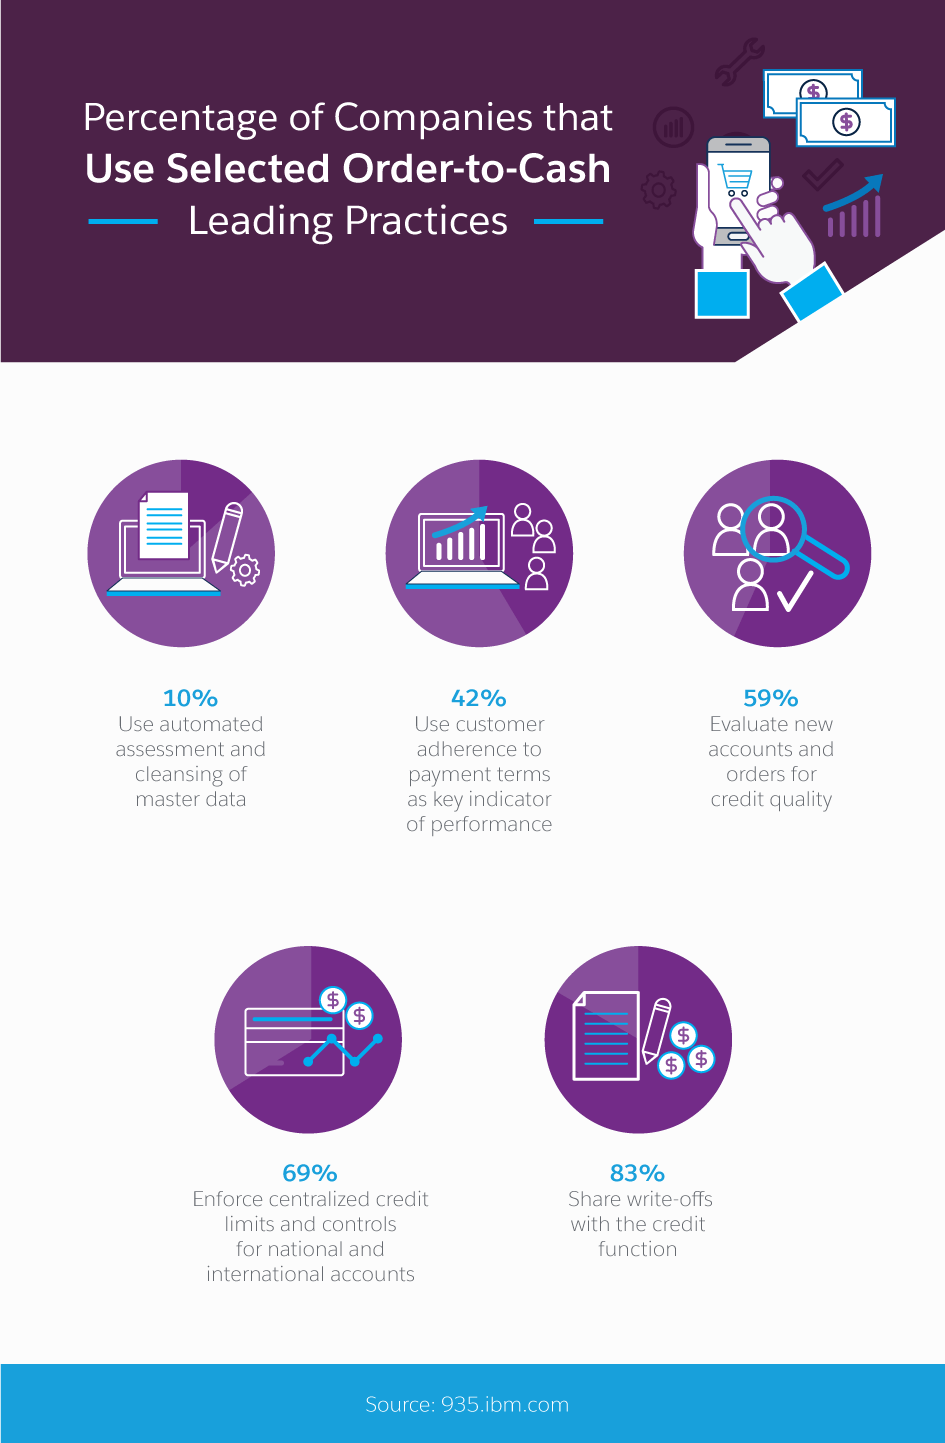
\includegraphics[width=10cm]{wong.png}
	\caption{Het aantal bedrijven dat gebruik maakt van order-to-cash proces. \textcite{Wong2018}}
	\centering
\end{figure}
  
Bij een OTC is technologie cruciaal. Elk deeltje van het proces kan beter worden door een correcte implementatie van microservices. Microservices kunnen hierbij helpen. Ze kunnen ervoor zorgen dat de automatisering vlotter verloopt.

In figuur 2.15 wordt het afgebeeld in een schema.
\begin{figure}[h!]
	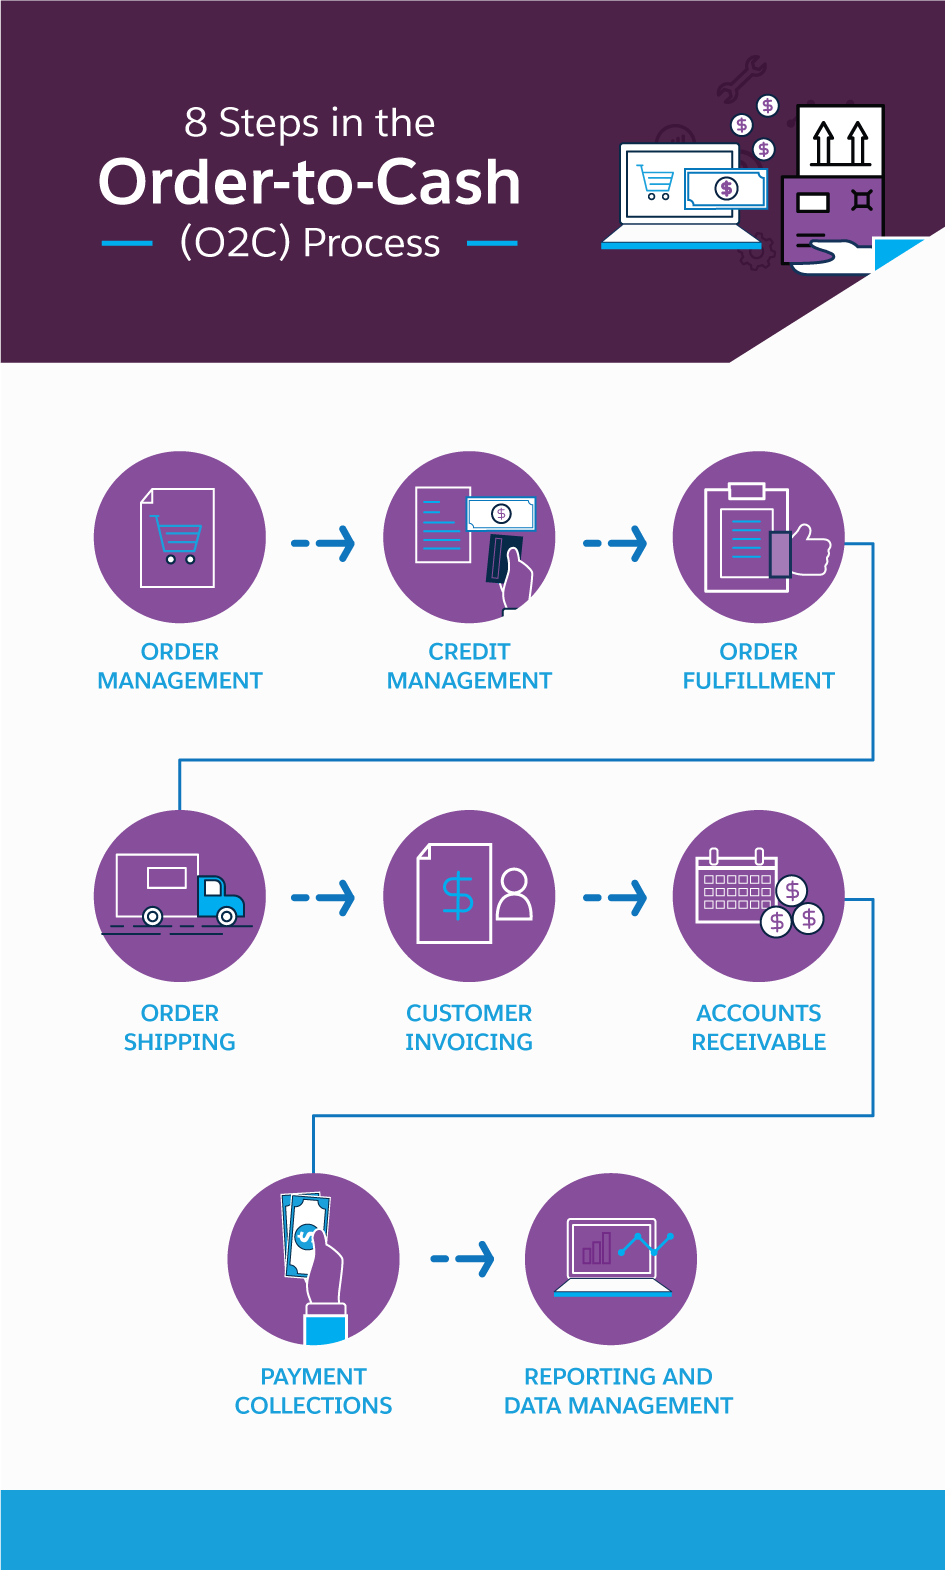
\includegraphics[width=10cm]{wong2.png}
	\caption{Het order-to-cash proces. \textcite{Wong2018}}
	\centering
\end{figure}


\subsection{Technologie: Wat biedt SAP zelf aan voor microservices}
SAP biedt een open-source project aan genaamd Kyma om microservices te implementeren.
Kyma maakt de werking met microserivces eenvoudige. Kubernetes wordt gebruikt om applicaties op verschillende machines te managen. Het kan onder meer gebruikt worden om cloud-based en on-premise applicaties om te zetten naar een microservice architectuur. Cloud-based applicaties zijn applicaties die hun data gaan ophalen op het internet in plaats van op de harde schijf van de computer. On-premise is lokaal op de computer, op de harde schijf. Kyma zorgt voor betere end-to-end ervaring voor scenario's, \textcite{Kyma2019}.

Binnen SAP wordt er omgegaan met software van verschillende leveranciers. SAP probeert om hun software te customizen naar de  wensen van de klant. Dit vraagt meer openheid en een modernere architectuur. 
Het idee achter Kyma is het creëeren van serverless applicaties, mashups en microservices. Het kan  gebruikt worden om snel kleine, gecustomizede modules te ontwikkelen. 

Knative is een platform dat developers ondersteunt om serverless applicaties te maken op Kubernetes en samenwerkt met Kyma. Dit zorgde voor groot enthousiasme bij SAP omdat hun Kyma project een bevesteging kreeg. Al snel  werd Kyma gerefactored om samen te kunnen  werken met Knative. Er werden overlappende componenten  weggelaten, wat Kyma slanker en gestroomlijnder maakt. Dankzij Knative kan Kyma zich richten op higer-level enterprise applications en service consumption scenario's, \textcite{Semerdzhiev2018}.

De samenwerking tussen Kyma en Knative is belangrijk. Er wordt een complete set van bouwblokken aangeboden en het zijn twee sterke frameworks. Bij het gebruik van beide kunnen er could-native oplossingen gebouwd worden op Kubernetes met een sterk framework. Op figuur 2.16 is te zien wat Kyma en Knative aanbiedt. \textcite{Hofmann2018}
\begin{figure}[h!]
	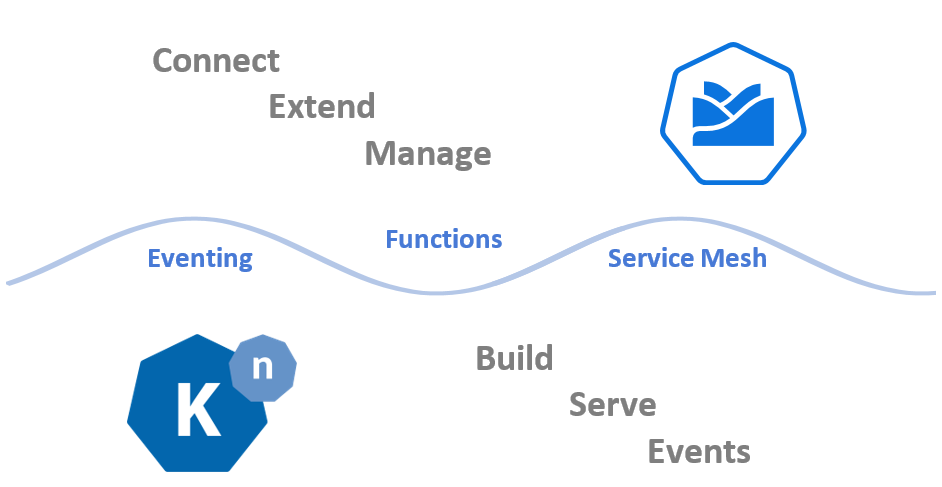
\includegraphics[width=10cm]{1-kyma-knative.png}
	\caption{Wat Kyma, boven de lijn, aanbiedt en wat Knative, onder de lijn, aanbiedt \textcite{Hofmann2018}.}
	\centering
\end{figure}


\section{Requirements van de business}
Het OTC proces heeft volgende nodig van een bedrijf, \textcite{Biedron2018}
\begin{itemize}
	\item De klant moet een order of meerdere orders kunnen plaatsen. Een goed werkend order-systeem is een must.
	\item Het order ophalen uit de voorraad. Er moet een goed voorraadbeheer aanwezig zijn. Dit moet ervoor zorgen dat het aantal laattijdige leveringen geminimaliseerd wordt. Samen met een goed voorraadbeheer wordt ook best bijgehouden waar men goederen geplaatst heeft in het magazijn.
	\item De levering moet goed gepland worden. Dit zou voor het grootste deel al geautomatiseerd moeten zijn. Een email met informatie over de levering is hierbij een verplichting. 
	\item Aanmaken van een factuur op basis van het geplaatst order met de juiste klantgegevens moet geautmatiseerd onderdeel worden. 
	\item De betaling van de factuur komt toe in de financiele afdeling. Automatische afhandeling is een verplicting.
\end{itemize}
Bij een order plaatsen komen volgende elementen aanbod:
\begin{itemize}
	\item Er moet een lijst met producten beschikbaar zijn.
	\item De klant zijn gegevens moeten gekend zijn bij het bedrijf.
	\item Het systeem bij het bedrijf moet beschikbaar zijn.
\end{itemize}
Na het plaatsen van het order die klaargezet worden om te leveren. Daar zijn volgende elementen van belang:
\begin{itemize}
	\item Een goed voorraadbeheer is de eerste must.
	\item Een overzicht van waar alles staat, geeft een meerwaarde.
	\item Bij het ophalen van een product om bij een order te plaatsen, moet de hoeveelheid in de voorraad verminderen.
\end{itemize}
